\documentclass[a0paper,25pt,portrait,blockverticalspace=20mm, colspace=20mm]{tikzposter}

\usepackage{etex}

\usepackage{amsmath,amsthm,mathrsfs,amssymb,amsfonts,dsfont,nicefrac,stmaryrd,yhmath}
\usepackage{mathtools,cancel}
\mathtoolsset{showonlyrefs=true}

\usepackage{multicol}
\usepackage{subfigure}

\usepackage{bold-extra,moresize}

\usepackage{layout}

\usepackage{pgfplots}
\pgfplotsset{compat=newest}
%\usetikzlibrary{plotmarks}

\usetikzlibrary{arrows,positioning,shapes} 
\usetikzlibrary{datavisualization}
\usetikzlibrary{arrows,positioning,shapes,trees,mindmap,shadows} 
\usepackage{pgfpages}
\usepackage{tikz-3dplot}

%%%%%%%%%%%%%
%
% Defining commands
%
%%%%%%%%%%%%%


\newcommand{\R}{\mathbb{R}}
\newcommand{\C}{\mathbb{C}}
\newcommand{\Q}{\mathbb{Q}}
\newcommand{\N}{\mathbb{N}}
\newcommand{\Z}{\mathbb{Z}}
\newcommand{\K}{\mathbb{K}}
\newcommand{\Y}{\mathbb{Y}}

\renewcommand{\H}{\mathbb{H}}
\newcommand{\V}{\mathbb{V}}

\newcommand{\dis}{\displaystyle}
\newcommand{\abs}[1]{\left|#1\right|}
\newcommand{\eps}{\varepsilon}
\newcommand{\norme}[1]{\left\|#1\right\|}
\newcommand{\norm}[1]{\left\|#1\right\|}

\renewcommand{\leq}{\leqslant}
\renewcommand{\geq}{\geqslant}
\renewcommand{\tilde}{\widetilde}
\newcommand{\grad}{\nabla}
\newcommand{\scalaire}[2]{\left<#1\,,#2\right>}


%
%
%%%%%%%%%%%%
%
% Redefining style
%
%%%%%%%%%%%%%%
\tikzposterlatexaffectionproofoff
%\usetheme{Wave}

\definecolor{myred}{rgb}{0.5,0,0.1}
\definecolor{mygreen}{rgb}{0,0.5,0.1}
\definecolor{mybrown}{rgb}{0.75,0.5,0}
\definecolor{mygray}{rgb}{0.5,0.5,0.5}
 \definecolorstyle{myColorStyle}{%
\colorlet{colorOne}{mygreen}
 \colorlet{colorTwo}{mygray} 
 \colorlet{colorThree}{mybrown}
 %
}{
% Background Colors 
\colorlet{backgroundcolor}{colorOne!50} 
\colorlet{framecolor}{colorTwo!50}
% Title Colors 
\colorlet{titlefgcolor}{black} 
\colorlet{titlebgcolor}{colorOne!60}
% Block Colors 
\colorlet{blocktitlebgcolor}{colorThree!60} 
\colorlet{blocktitlefgcolor}{black} 
\colorlet{blockbodybgcolor}{colorTwo!5} 
\colorlet{blockbodyfgcolor}{black}
% Innerblock Colors
\colorlet{innerblocktitlebgcolor}{colorOne!60} 
\colorlet{innerblocktitlefgcolor}{black} 
\colorlet{innerblockbodybgcolor}{colorOne!20} 
\colorlet{innerblockbodyfgcolor}{black}
% Note colors 
\colorlet{notefgcolor}{black} 
\colorlet{notebgcolor}{yellow!50} 
\colorlet{notefrcolor}{white}
}

\usecolorstyle{myColorStyle}
%\usecolorstyle[colorPalette=GreenGrayViolet]{Russia}
\usebackgroundstyle{BottomVerticalGradation}
\usenotestyle{Corner}

\usetitlestyle{Wave}
\useblockstyle{Envelope}

%\newlength{\logoheight}
%\setlength{\logoheight=2cm}

\newlength{\plotwidth}
\newlength{\plotheight}


\newcommand{\todoVD}[2][]%
{\todo[color=green!25,#1]{\footnotesize{\bf Vincent:} #2}}

\newcommand{\todoJA}[2][]%
{\todo[color=cyan!25,#1]{\footnotesize{\bf Julen:} #2}}

\newcommand{\todoDP}[2][]%
{\todo[color=blue!25,#1]{\footnotesize{\bf David:} #2}}

\newcommand{\todoFC}[2][]%
{\todo[color=red!25,#1]{\footnotesize{\bf Felipe:} #2}}

%%%%%%%%%%%%%%%%%%%
\usetikzlibrary{matrix,chains,positioning,decorations.pathreplacing,arrows}
%%%%%%%%%%%%%%%%%%%%%%%% tikz packaque
%\usepackage{tikz}
\usetikzlibrary{shapes.geometric, arrows}
\tikzstyle{startstop} = [rectangle, rounded corners, minimum width=3cm, minimum height=1cm,text centered, draw=black, fill=red!30]
\tikzstyle{process} = [rectangle, minimum width=1cm, minimum height=1cm, text centered, draw=black, fill=orange!30]
\tikzstyle{process_2} = [rectangle, minimum width=2cm, minimum height=1cm, text centered, text width=4cm, draw=black, fill=orange!30]
\tikzstyle{process_3} = [rectangle, minimum width=2cm, minimum height=1cm, text centered, text width=2cm, draw=black, fill=orange!30]
\tikzstyle{process_4} = [rectangle, minimum width=1cm, minimum height=1cm, text centered, text width=1.2cm, draw=black, fill=orange!30]
\tikzstyle{arrow} = [thick,->,>=stealth]
%%%%%%%%%%%%%%%%%%%
\newcommand{\mbbU}{\mathbb{U}}
\newcommand{\mbbV}{\mathbb{V}}
\newcommand{\mbbR}{\mathbb{R}}
\DeclareMathOperator*{\argmin}{argmin}
%%%%%%%%%%%%%%%%%%%

\title{\parbox{\linewidth}{\centering A Machine Learning Minimal Residual Method for Solving Quantities of Interest of Parametric PDEs}}
\titlegraphic{

\includegraphics[height=4.6cm]{Figures/UoN_logo.png} \quad 

\includegraphics[height=4.6cm]{Figures/IMA_PUCV_logo.png} \quad

\includegraphics[height=4.6cm]{Figures/logo_bcam_v2.png} \quad 

\includegraphics[height=4.6cm]{Figures/UPV-EHU-logo_v2.png} \quad

\includegraphics[height=4.6cm]{Figures/EPSRC_logo.png}
}

\author{{{\bf Ignacio Brevis}, Ignacio Muga, David Pardo, Oscar Rodr\'iguez, and Kristoffer G. van der Zee}}
%\institute{MathMode}
\settitle{ \centering \vbox{
     \centering
     \color{titlefgcolor} {\bfseries \Huge \@title \par}
     \vspace*{1em}
     {\LARGE \it \@author \par} \vspace*{1em}  \@titlegraphic \\[\TP@titlegraphictotitledistance]\vspace*{-1em} {\Large \@institute}
}}

% !TEX root = poster.tex
\tikzset{mark size=3}

\newcommand{\PbName}{}
\newcommand{\ColName}{}
\newcommand{\FigurePath}{Figures}
\newcommand{\DataPath}{}

%==========
% \errorplotlog
%==========
\newcommand{\errorplotlog}[3][]{

  \renewcommand{\DataPath}{\FigurePath/#2}
  \renewcommand{\PbName}{#2}
  \renewcommand{\ColName}{#3} 
  
  %\findmax{\DataPath/h/order_2/outputs.txt}{nr_dof}{\maxdof}
  %\findmin{\DataPath/h/order_2/outputs.txt}{nr_dof}{\mindof}
  %\findmaxDbl{\DataPath/hp/order_1/outputs.txt}{Error}{\maxerror}
  %\findminDbl{\DataPath/hp/order_1/outputs.txt}{Error}{\minerror}

  \tikzset{/tikz/external/export next=false}
  \begin{tikzpicture}
    \pgfplotsset{xmode=log}

    \begin{axis}[width=\plotwidth,height=\plotheight,
		xlabel={Number of DoFs},
		%x dir=reverse,
		ylabel=Relative error in \% (log scale),
		ymode=log,
		xmode=log,
		%ymin=\minerror,
		%ymax=\maxerror,
		%xmin=\mindof,
		%xmax=\maxdof,
		ytick={0.0000001, 0.0001, 0.1, 100},
		%extra y ticks={\minerror,\maxerror},
		%yticklabel pos=right,
		ylabel near ticks,
		xlabel near ticks,
		enlargelimits=true,
		legend style={draw=black,fill=white,legend cell align=left, at={(0.5,1.01)}, anchor=south},
		legend columns=-1
		]
		\addplot+[ line width=1pt] table[x expr=\thisrow{nr_dof},y expr=\thisrow{#3}] {\FigurePath/\PbName/hp/order_1/outputs.txt}node[pos=0.9, pin={[pin edge=solid]180:$hp$}]{};
		
		\addplot+[ line width=1pt] table[x expr=\thisrow{nr_dof},y expr=\thisrow{#3}] {\FigurePath/\PbName/h/order_1/outputs.txt}node[pos=0.9, pin={[pin edge=solid]90:$h$ ($p=1$)}]{};
		
		\addplot+[ line width=1pt] table[x expr=\thisrow{nr_dof},y expr=\thisrow{#3}] {\FigurePath/\PbName/h/order_2/outputs.txt} node[pos=0.9, pin={[pin edge=solid]-90:$h$ ($p=2$)}]{};
    \end{axis}
  \end{tikzpicture}
} 
%======
% \plothp
%======
\newcommand{\plothp}[2][]{

  \renewcommand{\DataPath}{\FigurePath/#2/hp/order_1}%\PbName/hp
  \findmax{\DataPath/outputs.txt}{iter}{\endIter}
  
   \FormatIntegerThreeDigit{\endIter}{\endIterformated}
   
    %\centering
    \begin{minipage}[b]{0.45\linewidth}
    \raggedleft
    %\begin{tikzfigure}[Final $hp$-adapted mesh with polynomial orders in the $x$-direction.]
    \plothpmesh{#2/hp/order_1}{\endIterformated}{X}
    %\end{tikzfigure}%
    \end{minipage} \quad
    \begin{minipage}[b]{0.45\linewidth}
    \raggedright
    %\begin{tikzfigure}[Final $hp$-adapted mesh with polynomial orders in the $y$-direction.]
     \plothpmesh{#2/hp/order_1}{\endIterformated}{Y}
    %\end{tikzfigure}%
    \end{minipage}% 
}

\newcommand{\plothpmesh}[3]{
  \renewcommand{\DataPath}{\FigurePath/#1}

  \lastelement{\DataPath/outputs.txt}{MaxP}{\maxp}
  \lastelement{\DataPath/outputs.txt}{MinP}{\minp}

  \pgfplotsset{colormap/YlOrRd} 
  \tikzset{/tikz/external/export next=false}
  \begin{tikzpicture}
    \begin{axis}[name=master,
        width=0.95\textwidth,height=0.95\textwidth,
        enlargelimits=false,
        xlabel=$x$,
        ylabel=$y$,
        xlabel near ticks,
        ylabel near ticks,
        xtick={0,0.5,1},
        ytick={0,0.5,1},
        colorbar horizontal,
        colorbar style={%
            xtick={1,2,...,\maxp},
            title={Order of approximation},
            at={(master.above north west)},anchor=south west,
            yshift=-5pt,
            title style={
                yshift=20pt
              },
            yshift=0.1em,
            xticklabel pos=upper,
          },
        %point meta min=\minp,
        point meta min=1,
        point meta max=\maxp,
      ]
      %
      \addplot [forget plot] graphics[xmin=0,xmax=1,ymin=0,ymax=1] {\DataPath/mesh_#3_#2.png};

    \end{axis}
  \end{tikzpicture}
}
%===============
% elemental routines
%===============
\newcommand{\FormatIntegerTwoDigit}[2]{
\pgfmathsetbasenumberlength{2}
\pgfmathbasetodec#2{#1}{10}
}

\newcommand{\FormatIntegerThreeDigit}[2]{
\pgfmathsetbasenumberlength{3}
\pgfmathbasetodec#2{#1}{10}
}

\newcommand{\getelem}[4]{
    \pgfplotstablegetelem{#3}{#2}\of{#1}%
    \pgfmathtruncatemacro#4{\pgfplotsretval}
    \pgfplotstableclear{\datatable}
}


\newcommand{\getelemdbl}[4]{
    \pgfplotstablegetelem{#3}{#2}\of{#1}%
    \pgfmathsetmacro#4{\pgfplotsretval}    
    \pgfplotstableclear{\datatable}
}



\newcommand{\findmax}[3]{
  \pgfplotstableread{#1}{\datatable}
  \pgfplotstablesort[sort key={#2},sort cmp={float >}]{\sorted}{\datatable}%
  \pgfplotstablegetelem{0}{#2}\of{\sorted}%
  \pgfmathtruncatemacro#3{\pgfplotsretval}
  \pgfplotstableclear{\datatable}
}

\newcommand{\findmin}[3]{
  \pgfplotstableread{#1}{\datatable}
  \pgfplotstablesort[sort key={#2},sort cmp={float <}]{\sorted}{\datatable}%
  \pgfplotstablegetelem{0}{#2}\of{\sorted}%
  \pgfmathtruncatemacro#3{\pgfplotsretval}
  \pgfplotstableclear{\datatable}
  %
}

\newcommand{\findmaxDbl}[3]{
  \pgfplotstableread{#1}{\datatable}
  \pgfplotstablesort[sort key={#2},sort cmp={float >}]{\sorted}{\datatable}%
  \pgfplotstablegetelem{0}{#2}\of{\sorted}%
  \pgfmathsetmacro#3{\pgfplotsretval}
  \pgfplotstableclear{\datatable}
  %
}

\newcommand{\lastelement}[3]{
\pgfplotstableread{#1}{\mytable}
\pgfplotstablegetrowsof{\mytable} %Determine no. of rows
\pgfmathtruncatemacro{\rows}{\pgfplotsretval}
\pgfmathtruncatemacro{\lastrow}{\rows-1}
\pgfplotstablegetelem{\lastrow}{#2}\of{\mytable}
\pgfmathsetmacro#3{\pgfplotsretval}
}


\newcommand{\findminDbl}[3]{
  \pgfplotstableread{#1}{\datatable}
  \pgfplotstablesort[sort key={#2},sort cmp={float <}]{\sorted}{\datatable}%
  \pgfplotstablegetelem{0}{#2}\of{\sorted}%
  \pgfmathsetmacro#3{\pgfplotsretval}
  \let#3=\pgfplotsretval
  \pgfplotstableclear{\datatable}
  %
}

\pgfplotsset{
  log x ticks with fixed point/.style={
      xticklabel={
        \pgfkeys{/pgf/fpu=true}
        \pgfmathparse{exp(\tick)}%
        \pgfmathprintnumber[fixed relative, precision=3]{\pgfmathresult}
        \pgfkeys{/pgf/fpu=false}
      }
  },
  log y ticks with fixed point/.style={
      yticklabel={
        \pgfkeys{/pgf/fpu=true}
        \pgfmathparse{exp(\tick)}%
        \pgfmathprintnumber[fixed relative, precision=3]{\pgfmathresult}
        \pgfkeys{/pgf/fpu=false}
      }
  }
}

\pgfplotscreateplotcyclelist{custom list style}{%
color=red, solid, every mark/.append style={solid}, mark=*\\%
color=blue, loosely dotted, every mark/.append style={solid}, mark=triangle*\\%
color=black!50!green,dotted, every mark/.append style={solid}, mark=square*\\%
color=black, dashed, every mark/.append style={solid},mark=diamond*\\%
color=black!50!red, densely dotted, every mark/.append style={solid}, mark=otimes*\\%
color=black!50!yellow, loosely dashed, every mark/.append style={solid},mark=*\\%
color=black!50!blue,densely dashed, every mark/.append style={solid},mark=square*\\%
color=black!50!magenta,dashdotted, every mark/.append style={solid},mark=otimes*\\%
color=black!50!orange,dashdotdotted, every mark/.append style={solid},mark=star\\%
color=black!50!cyan, densely dashdotted,every mark/.append style={solid},mark=diamond*\\%
}

\pgfplotsset{%
%    every axis plot/.append style= {line width=2pt},
        every axis plot/.append style= ultra thick,
    cycle list name=custom list style,
%    log x ticks with fixed point,
%    legend style={at={(0.5,1.03)},anchor=south},
%    legend columns=3,
%    legend pos= outer north east,
%    legend cell align=left,
    }
 
\begin{document} 
\maketitle
%%%%%%%%%%%%%%%%%%%%%%%%%%%%%%%%%%%%%%%%%%%%%%%%%%%%%%%%%%%%%%%%
\begin{columns}
%
\column{0.5} 
%
\block{Problem definition}{ %
We want:
\begin{itemize}
\item Solve parametric families of PDEs
\item High precision in terms of a Quantity of Interest (QoI)
\item Employing coarse meshes in Finite Elements
\end{itemize}
\innerblock{}{
We consider the abstract variational formulation:\\
Given $\lambda\in\Lambda\subset\mathbb R^p$, find $q(u) \in \mathbb{R}$ such that 
\begin{equation}
\left\{
\begin{array}{l}
 u\in \mbbU \text{ solves:} \\
B_{\lambda} u  = \ell_{\lambda} \quad \in \mbbV^*, %\quad \forall\, \lambda \in \Lambda.
\end{array}
\right.
\quad \Leftrightarrow\quad 
\left\{
\begin{array}{l}
 u\in \mbbU \text{ solves:} \\
b_{\lambda}(u,v) = \ell_{\lambda}(v), \quad \forall\, v \in \mbbV. 
\end{array}
\right.
\label{eq:continuous_variational_formulation}
\end{equation}
}
%
%For any element $K$, we denote by $\calR_K$ the set of \emph{removable} basis functions associated to $K$, by $\abs{\calR_K}$ its cardinality, and by $\H_{\calR_K}$ its associated space.
We will use:
\begin{itemize}
\item Minimal-residual (MinRes) finite elements
\item Artificial neural networks
\end{itemize}
}
%%%%%%%%%%%%%%%%%%%%%%%%%%%%%%%%%%%%%%%%%%%%%%%%%%%%%%%%%%%%%%%%%%%%%%%%%%
\block{Introduction to the method (weighted-MinRes)}{ %
Given discrete conforming trial $\mbbU_n := \text{span}\{ \varphi_1,\dots, \varphi_n\} \subset \mbbU$, and test $\mbbV_m \subset \mbbV$ spaces such that $\dim \mbbV_m > \dim \mbbU_n$, we want to find a discrete solution
\begin{equation}
u_{n} := \argmin_{w_n\in \mbbU_n} \| \ell_{\lambda} - B_{\lambda} w_n\|_{(\mbbV_m)^{*}}, \quad \text{\textcolor{red}{(MinRes method)}}
\label{eq:discrete_min_res}
\end{equation}
%
\innerblock{}{
To solve the above problem %~\eqref{eq:discrete_min_res}
is equivalent to solve the following saddle point problem:
\begin{equation}
\left\{ \begin{array}{rll}
\text{Find } (r_m, u_n) \in \mathbb{V}_m \times \mbbU_n &\text{ such that:} & \\
(r_m,v_m)_{\mbbV} + b_{\lambda}(u_n,v_m) &= \ell_\lambda(v_m), & \forall\, v_m \in \mbbV_m,\\
b_{\lambda}(w_n,r_m) &= 0 , & \forall\, w_n \in \mbbU_n.
\end{array} \right.
\label{eq:discrete_mixed_formulation}
\end{equation}
}
%
What we do:
%
%\vspace*{-28pt}
\begin{multicols}{2}
\innerblock{}{
We modify the MinRes method by introducing a \textcolor{red}{weighted inner product}
\begin{equation}
(\,\cdot\, , \cdot\,)_{\mbbV}\quad  \longrightarrow \quad (\,\cdot\, , \cdot\,)_{\textcolor{red}{\mbbV,\omega}}
\end{equation}
 in the $\mbbV$ space [$\,1\,$]
\vspace*{26pt}
}
\innerblock{}{
{\bf Example:} $H_{0}^{1}(\Omega)$
\begin{equation}
(r , v)_{\mbbV,\omega} = \sum_{k=1}^{K}  \omega_k \underbrace{\int_{\Omega_k} \nabla r(x) \cdot \nabla v(x)\, dx}_{G_k}
\end{equation}
}
\end{multicols}
%
\innerblock{}{
We seek for the coefficients $\omega :=(\omega_1,\dots,\omega_m)$, such that solving the system~\eqref{eq:discrete_mixed_formulation}
\begin{center}
$
\begin{array}{cl}
%\text{Find } (\alpha, \beta) \in \mbbR^{m} \times \mbbR^{n} \text{ s.t.:} & \\
\arraycolsep=1.4pt\def\arraystretch{1.2}
\left[\begin{array}{c|c}
G_\omega & B_\lambda \\
\hline
B_{\lambda}^{\top} & 0 
\end{array}
\right]
\left[\begin{array}{c}
\alpha \\ \hline \beta 
\end{array}
\right]
= 
\left[\begin{array}{c}
L_{\lambda} \\ \hline 0
\end{array}
\right], &
\end{array}$
\hspace*{3cm} with $\displaystyle G_\omega = \sum_{k=1}^{K} \omega_k G_k$.
\end{center}
delivers $u_{n}(x) :=\sum_{i=1}^{n} \beta_i(\omega) \varphi_i(x)$ as a good approximation for the QoI $q(u)$.
}
\innerblock{}{
{\bf Obs:} See [$\,2\,$] for an extension to Galerkin and least-squares formulations.
}
}
%%%%%%%%%%%%%%%%%%%%%%%%%%%%%%%%%%%%%%%%%%%%%%%%%%%%%%%%%%%%%%%%%%%%%%%%%%
\block{Artificial neural networks}{ %
We train a neural network $\text{nn}_\theta$ to learn the inner-product piecewise constant.
\begin{multicols}{2}
\innerblock{}{
\def\layersep{2.3cm}
Delivers every inner-product coefficient 
\begin{center}
\begin{tikzpicture}[shorten >=1pt,->,draw=black!50, node distance=\layersep]
    \tikzstyle{every pin edge}=[<-,shorten <=1pt]
    \tikzstyle{neuron}=[circle,draw=black,minimum size=26pt,inner sep=0pt]
    \tikzstyle{input neuron}=[neuron, fill=green!50];
    \tikzstyle{output neuron}=[neuron, fill=red!50];
    \tikzstyle{hidden neuron}=[neuron, fill=blue!50];
    \tikzstyle{annot} = [text width=4em, text centered]
    
    % Draw mesh
	%\draw[step=0.5cm, very thin,black!20] (-5,-5) grid (10,1);
    % Draw the input layer nodes
    \foreach \name / \y in {1}
    % This is the same as writing \foreach \name / \y in {1/1,2/2,3/3,4/4}
    	\node[neuron, pin=left:$\lambda$] (I-\name) at (-3.6cm,-1.8*\y cm) {};

    % Draw the hidden layer nodes
	\foreach \name / \y in {1,...,5}
        \path[yshift=1.2cm] %[yshift=1.587cm]
            node[neuron] (H1-\name) at (\layersep-3.6cm,-1.0*\y cm) {};    
    
    \foreach \name / \y in {1,...,5}
        \path[yshift=1.2cm]
            node[neuron] (H2-\name) at (2*\layersep-3.6cm,-1.0*\y cm) {};
            
    \foreach \name / \y in {1,...,5}
        \path[yshift=1.2cm]
            node[neuron] (H3-\name) at (3*\layersep-3.6cm,-1.0*\y cm) {};    
            
    \foreach \name / \y in {1,...,5}
        \path[yshift=1.2cm]
            node[neuron] (H4-\name) at (4*\layersep-3.6cm,-1.0*\y cm) {};    
    
        \path[yshift=3.2cm]
        	node[neuron,pin={[pin edge={->}]right:$\omega_1$}] (H6-2) at (5*\layersep-3.6cm,-2.0 cm) {};
        \path[yshift=3.2cm]
        	node (H6-3) at (5*\layersep-3.6cm,-3.0 cm) {};                        
        \path[yshift=3.2cm]
        	node[neuron,pin={[pin edge={->}]right:$\omega_2$}] (H6-4) at (5*\layersep-3.6cm,-4.0 cm) {};                        
        \path[yshift=3.2cm]
        	node (H6-5) at (5*\layersep-3.6cm,-5.0 cm) {};                        
        \path[yshift=3.2cm]
        	node (H6-6) at (5*\layersep-3.6cm,-6.0 cm) {$\vdots$};
        \path[yshift=3.2cm]
        	node (H6-7) at (5*\layersep-3.6cm,-7.0 cm) {};                        
        \path[yshift=3.2cm]
        	node[neuron,pin={[pin edge={->}]right:$\omega_K$}] (H6-8) at (5*\layersep-3.6cm,-8.0 cm) {};                        

    % Connect every node in the input layer with every node in the
    % hidden layer.
    \foreach \source in {1}
        \foreach \dest in {1,...,5}
            \path (I-\source) edge (H1-\dest);
            
    \foreach \source in {1,...,5}
        \foreach \dest in {1,...,5}
            \path (H1-\source) edge (H2-\dest);        

    \foreach \source in {1,...,5}
        \foreach \dest in {1,...,5}
            \path (H2-\source) edge (H3-\dest);   
            
    \foreach \source in {1,...,5}
        \foreach \dest in {1,...,5}
            \path (H3-\source) edge (H4-\dest); 
                            
    \foreach \source in {1,...,5}
        \foreach \dest in {2,4,8}
            \path (H4-\source) edge (H6-\dest);                                     

\end{tikzpicture}
\end{center}
}
%%%%%%%%%%%%%%%%%%%%%%%%%%%%%%%%%%%%%%%%%%%%%%%%%%%%%%%%%%%%%%%%%%%%%%%
%\innerblock{}{
%Delivers the $i$-th inner-product coefficient 
%\vspace*{34pt}
%\begin{center}
%\def\layersep{2.3cm}
%\begin{tikzpicture}[shorten >=1pt,->,draw=black!50, node distance=\layersep]
%    \tikzstyle{every pin edge}=[<-,shorten <=1pt]
%    \tikzstyle{neuron}=[circle,draw=black,minimum size=26pt,inner sep=0pt]
%    \tikzstyle{input neuron}=[neuron, fill=green!50];
%    \tikzstyle{output neuron}=[neuron, fill=red!50];
%    \tikzstyle{hidden neuron}=[neuron, fill=blue!50];
%    \tikzstyle{annot} = [text width=4em, text centered]
%    
%    % Draw mesh
%	%\draw[step=0.5cm, very thin,black!20] (-5,-5) grid (10,1);
%    % Draw the input layer nodes
%    %\foreach \name / \y in {1,2}
%    % This is the same as writing \foreach \name / \y in {1/1,2/2,3/3,4/4}
%    \node[neuron, pin=left:$\lambda$] (I-1) at (-3.6cm,-0.3cm - 1.0cm) {};
%    \node[neuron, pin=left:$i$] (I-2) at (-3.6cm,-0.3cm - 1.0*2 cm) {};
%
%    % Draw the hidden layer nodes
%	\foreach \name / \y in {1,...,5}
%        \path[yshift=1.2cm] %[yshift=1.587cm]
%            node[neuron] (H1-\name) at (\layersep-3.6cm,-1.0*\y cm) {};    
%    
%    \foreach \name / \y in {1,...,5}
%        \path[yshift=1.2cm]
%            node[neuron] (H2-\name) at (2*\layersep-3.6cm,-1.0*\y cm) {};
%            
%    \foreach \name / \y in {1,...,5}
%        \path[yshift=1.2cm]
%            node[neuron] (H3-\name) at (3*\layersep-3.6cm,-1.0*\y cm) {};    
%            
%    \foreach \name / \y in {1,...,5}
%        \path[yshift=1.2cm]
%            node[neuron] (H4-\name) at (4*\layersep-3.6cm,-1.0*\y cm) {};    
%                                                        
%        \path[yshift=3.2cm]
%        	node[neuron,pin={[pin edge={->}]right:$\omega_i\;\,$}] (H5-1) at (5*\layersep-3.6cm,-5.0 cm) {};                                           
%
%    % Draw the output layer node
%    %\node[neuron,pin={[pin edge={->}]right:Salida}, right of=H5-3] (O) {hola1};
%
%    % Connect every node in the input layer with every node in the
%    % hidden layer.
%    \foreach \source in {1,2}
%        \foreach \dest in {1,...,5}
%            \path (I-\source) edge (H1-\dest);
%            
%    \foreach \source in {1,...,5}
%        \foreach \dest in {1,...,5}
%            \path (H1-\source) edge (H2-\dest);        
%
%    \foreach \source in {1,...,5}
%        \foreach \dest in {1,...,5}
%            \path (H2-\source) edge (H3-\dest);   
%            
%    \foreach \source in {1,...,5}
%        \foreach \dest in {1,...,5}
%            \path (H3-\source) edge (H4-\dest);        
%         
%    \foreach \source in {1,...,5}
%        \path (H4-\source) edge (H5-1);                                     
%\end{tikzpicture}
%\end{center}
%}
%\vspace*{5pt}
\innerblock{}{
{\bf Training set}
\begin{equation}
\{\lambda^{(1)}, \lambda^{(2)},\dots \lambda^{(N_s)}\}
\end{equation}
}
\vspace*{10pt}
\innerblock{}{
{\bf Labels}
\begin{equation}
\{q(u_{\lambda^{(1)}}), q(u_{\lambda^{(2)}}),\dots q(u_{\lambda^{{(N_s)}}})\}
\end{equation}
}
\end{multicols}
%\begin{multicols}{2}
%\innerblock{Training set}{
%\begin{equation}
%\{\lambda_1, \lambda_2,\dots \lambda_{N_s}\}
%\end{equation}
%}
%\innerblock{Labels}{
%\begin{equation}
%\{q(u_{\lambda_1}), q(u_{\lambda_2}),\dots q(u_{\lambda_{N_s}})\}
%\end{equation}
%}
%\end{multicols}
\innerblock{Loss function}{
\begin{equation}
\mathcal{L}(\theta) := \frac{1}{N_s}\sum_{i=1}^{N_s}\frac{1}{2}\left|\frac{ q(u_{\lambda^{(i)}}) - q(u_{n,\lambda^{(i)}}(\theta))}{q(u_{\lambda^{(i)}})}\right|^2
\label{eq:loss_function}
\end{equation}
}
}
%%%%%%%%%%%%%%%%%%%%%%%%%%%%%%%%%%%%%%%%%%%%%%%%%%%%%%%%%%%%%%%%%%%%%%%%%%
\column{0.5} 
%
\block{Training process}{%
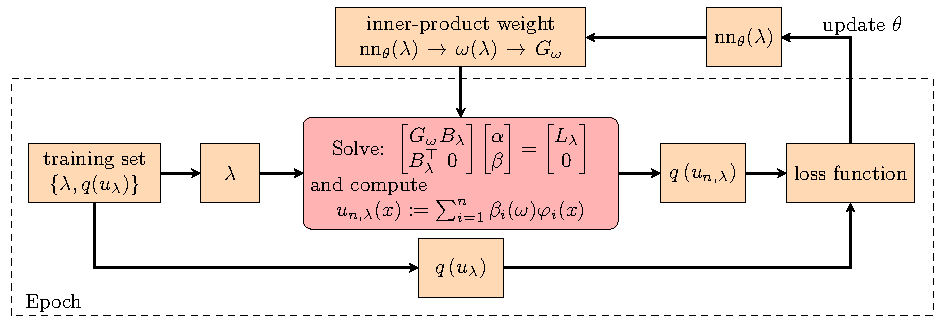
\includegraphics[width=0.45\textwidth]{Figures/NN/Training.pdf}
}
%%%%%%%%%%%%%%%%%%%%%%%%%%%%%%%%%%%%%%%%%%%%%%%%%%%%%%%%%%%%%%%%%%%%%%%%%%
\block{Ex: Diffusion with two parameters ($\dim \mbbU_n = 4$)}{
$$
\left\{
\begin{array}{rl}
- (a(x) u')' = 1, & \hbox{in } (0,1), \\
u(0) = u(1) = 0, &
\end{array}
\right.
\quad \text{with}\quad
a(x) = \begin{cases} \lambda_1, & \text{if } x \leq 0.5, \\  \lambda_2, & \text{if } x > 0.5. \end{cases}
\quad \text{and}\quad
q(u)= u(0.6)
$$ 
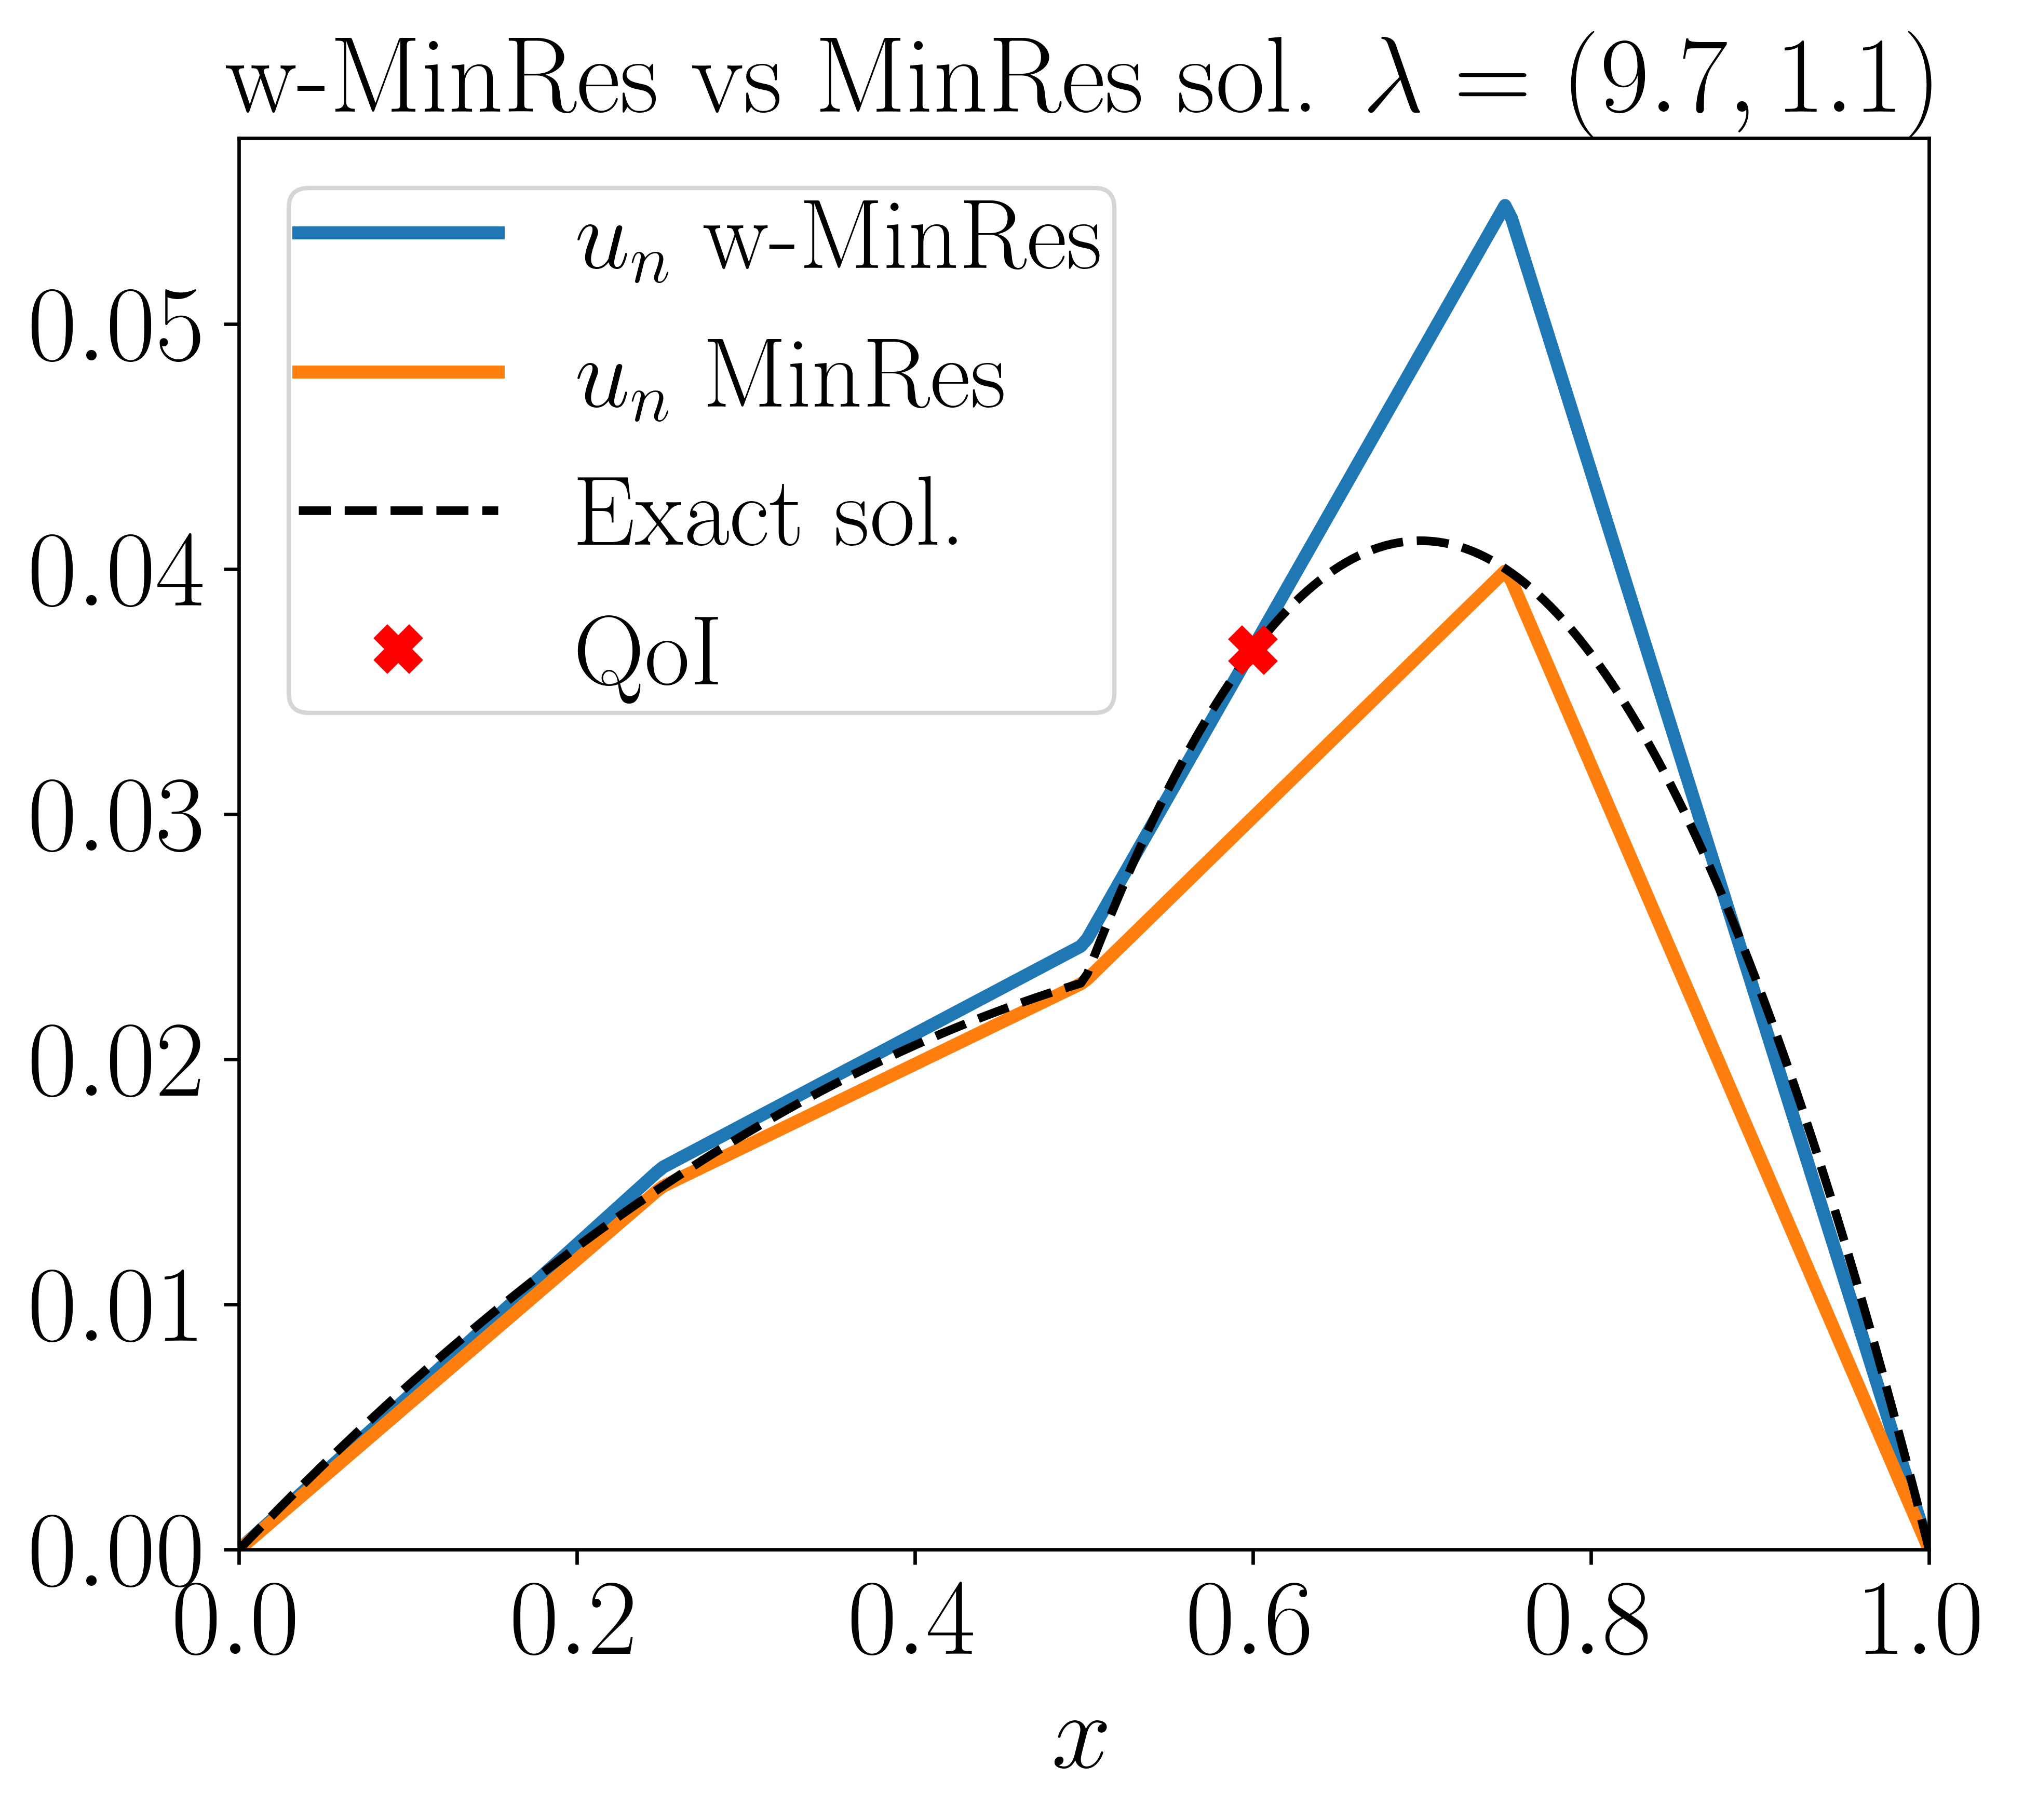
\includegraphics[scale=1.1]{Figures/diffusion_fig_02.png}
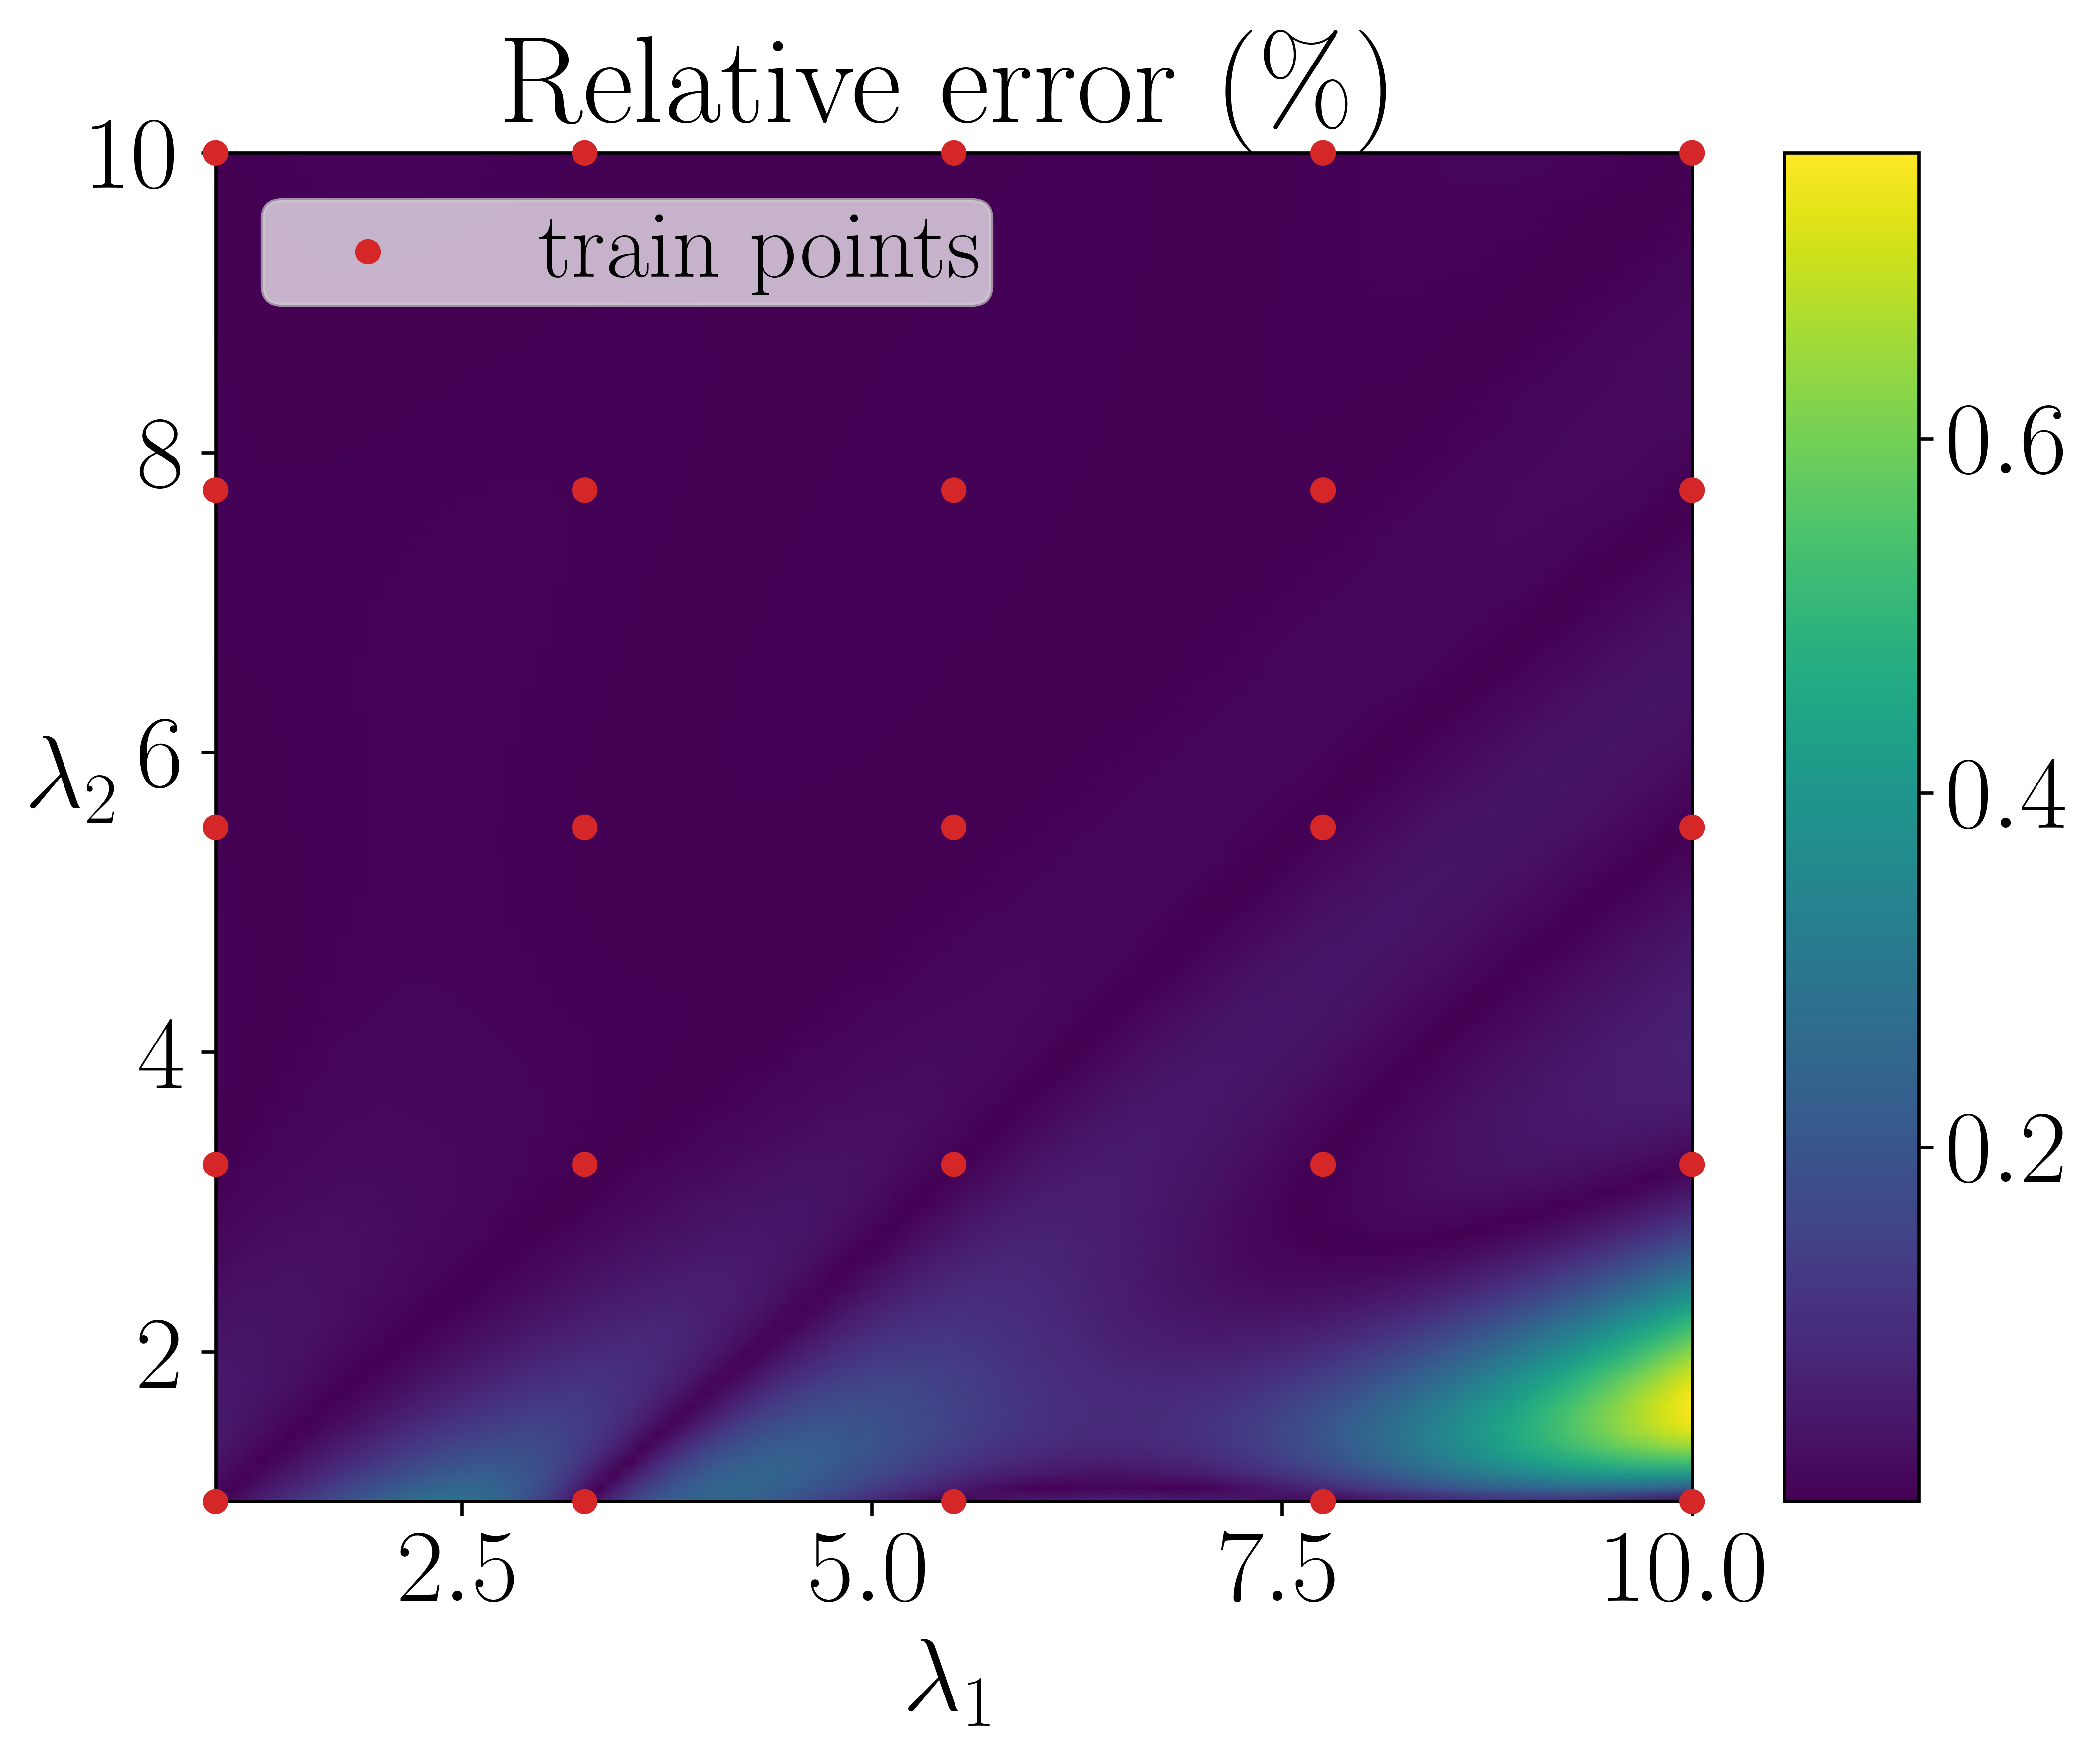
\includegraphics[scale=1.1]{Figures/output_POSTER.png}
}
%%%%%%%%%%%%%%%%%%%%%%%%%%%%%%%%%%%%%%%%%%%%%%%%%%%%%%%%%%%%%%%%%%%%%%%%%%
\block{Ex: Advection  with parametric rhs ($\dim \mbbU_n = 1$)}{
$$
\left\{
\begin{array}{rl}
 u' = f_{\lambda}, & \hbox{in } (0,1), \\
u(0) = 0, &
\end{array}
\right.
\quad \text{with}\quad
f_{\lambda}(x) = \begin{cases} 0, & \text{if } x \leq \lambda, \\  x - \lambda, & \text{if } x > \lambda. \end{cases}
\quad \text{and}\quad
q(u)= u(0.9)
$$ 
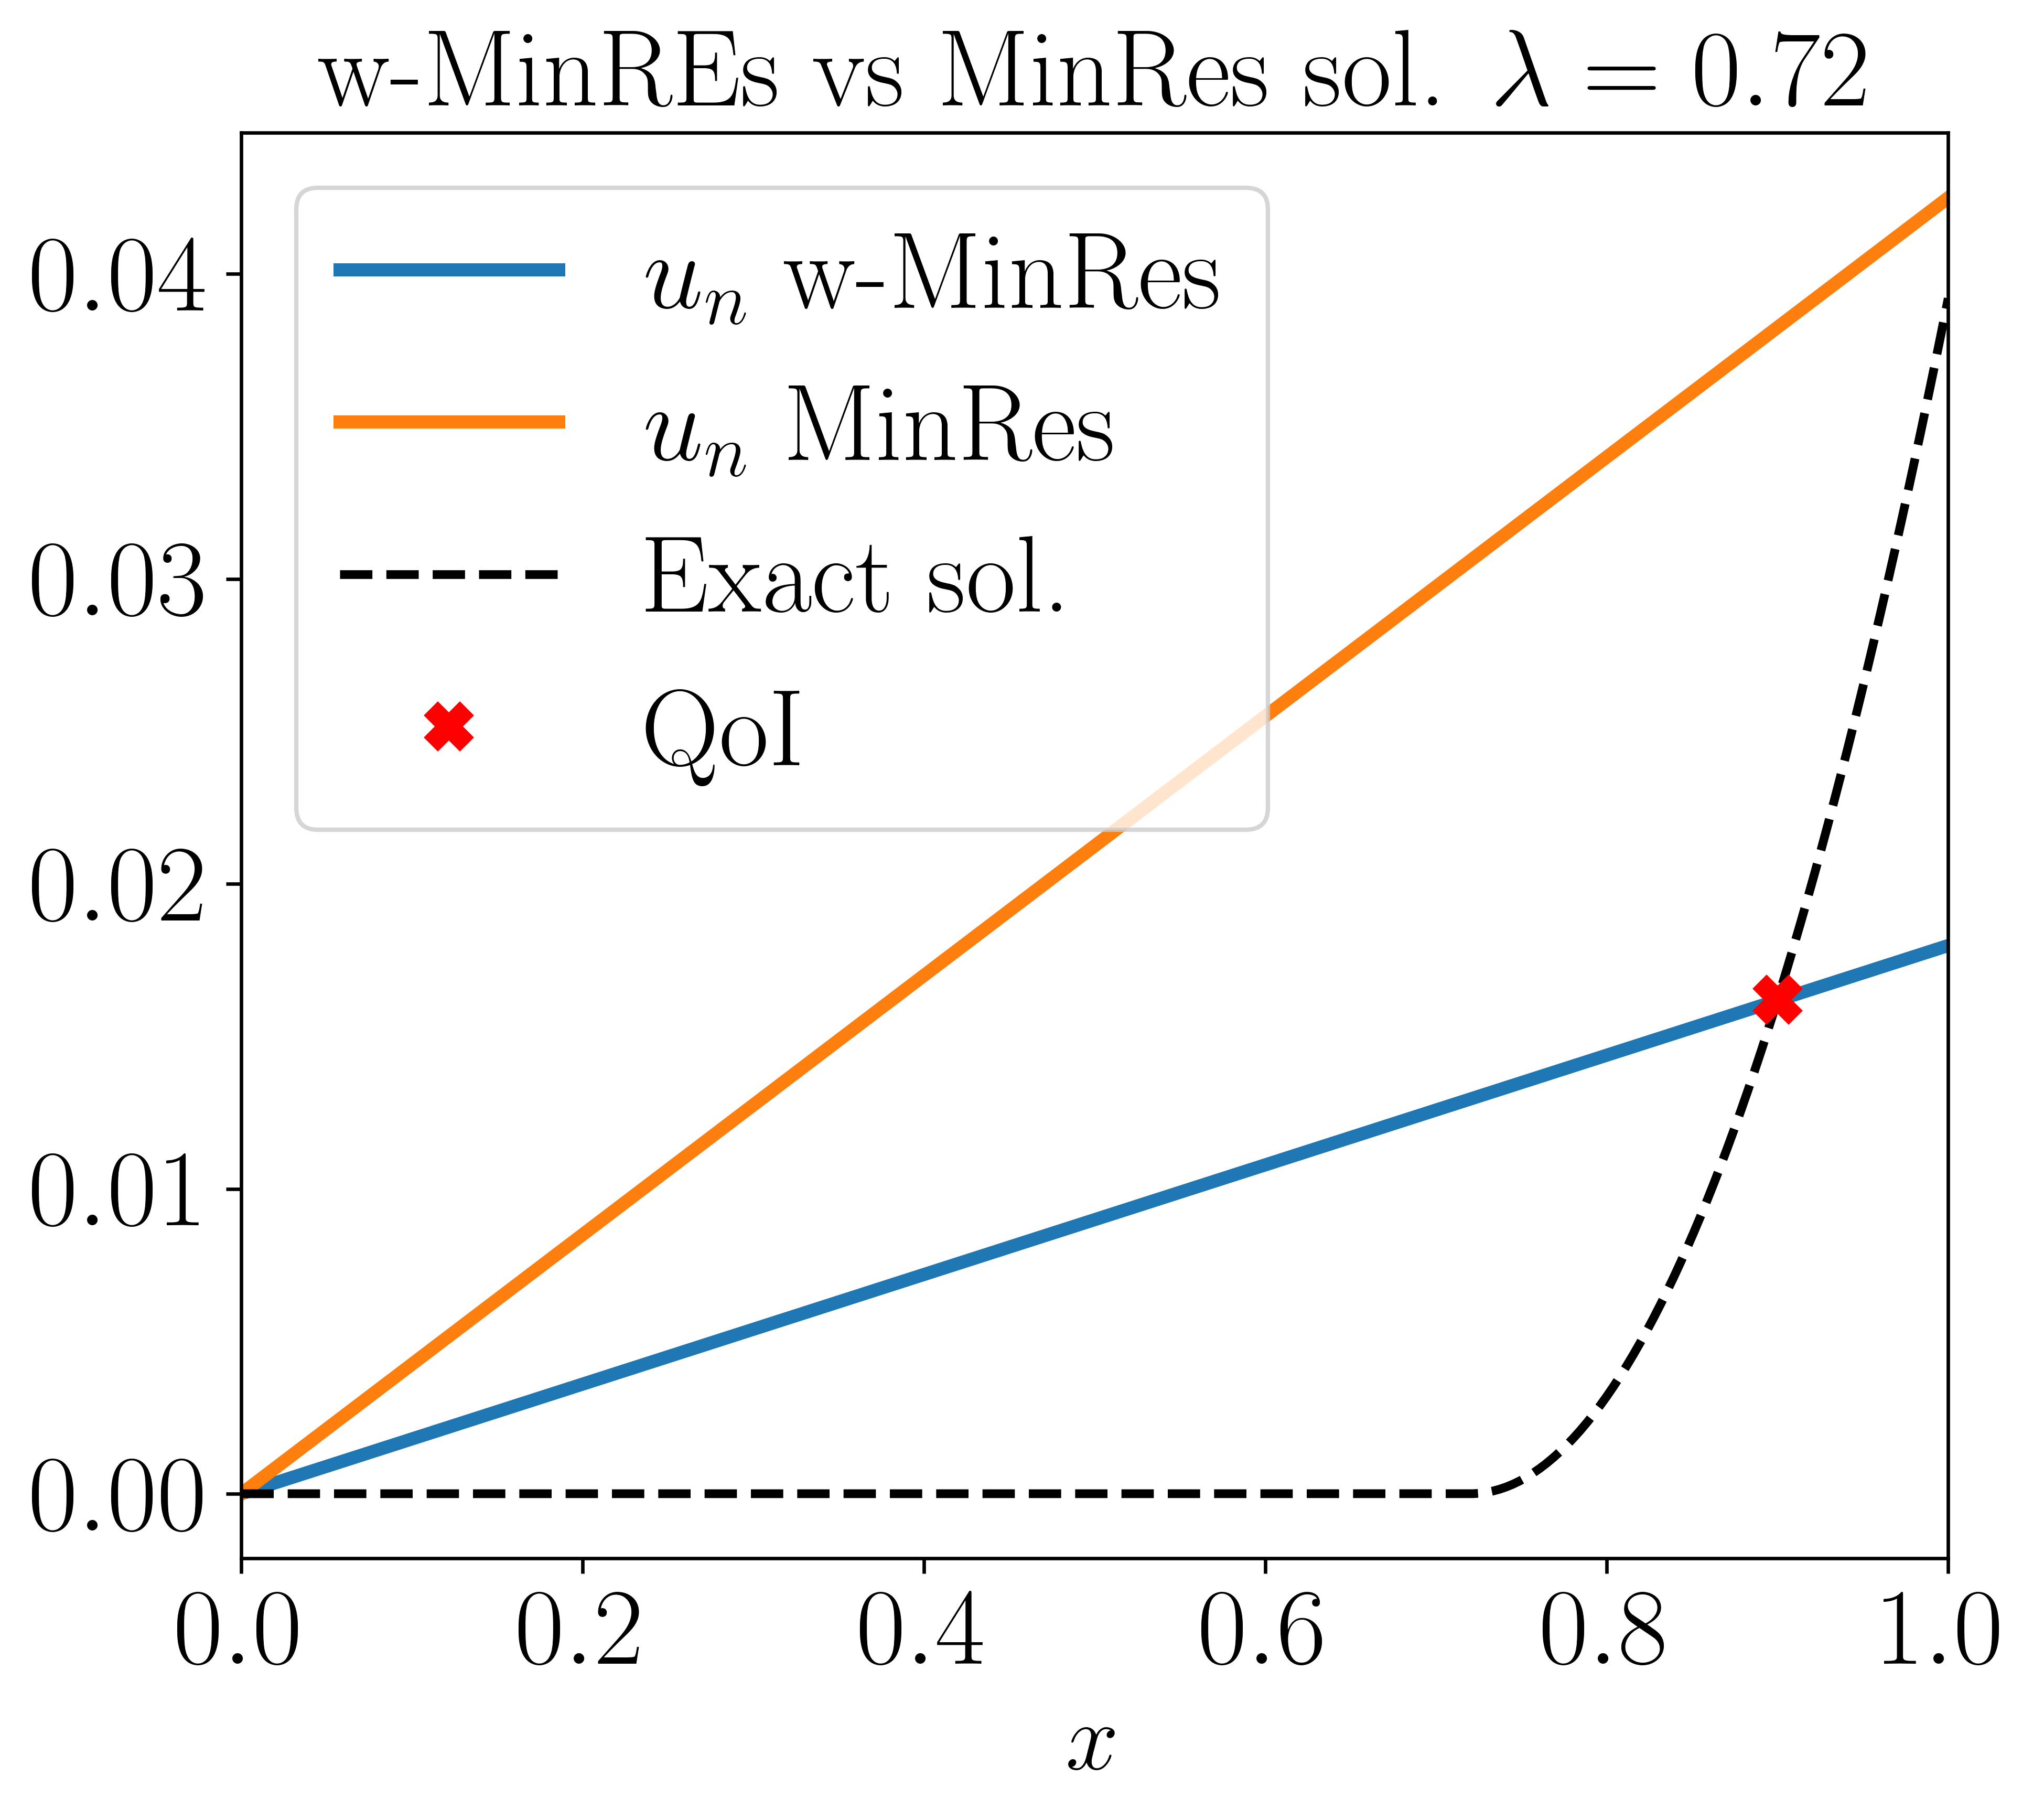
\includegraphics[scale=1.1]{Figures/ex2_single_POSTER_v2.png}
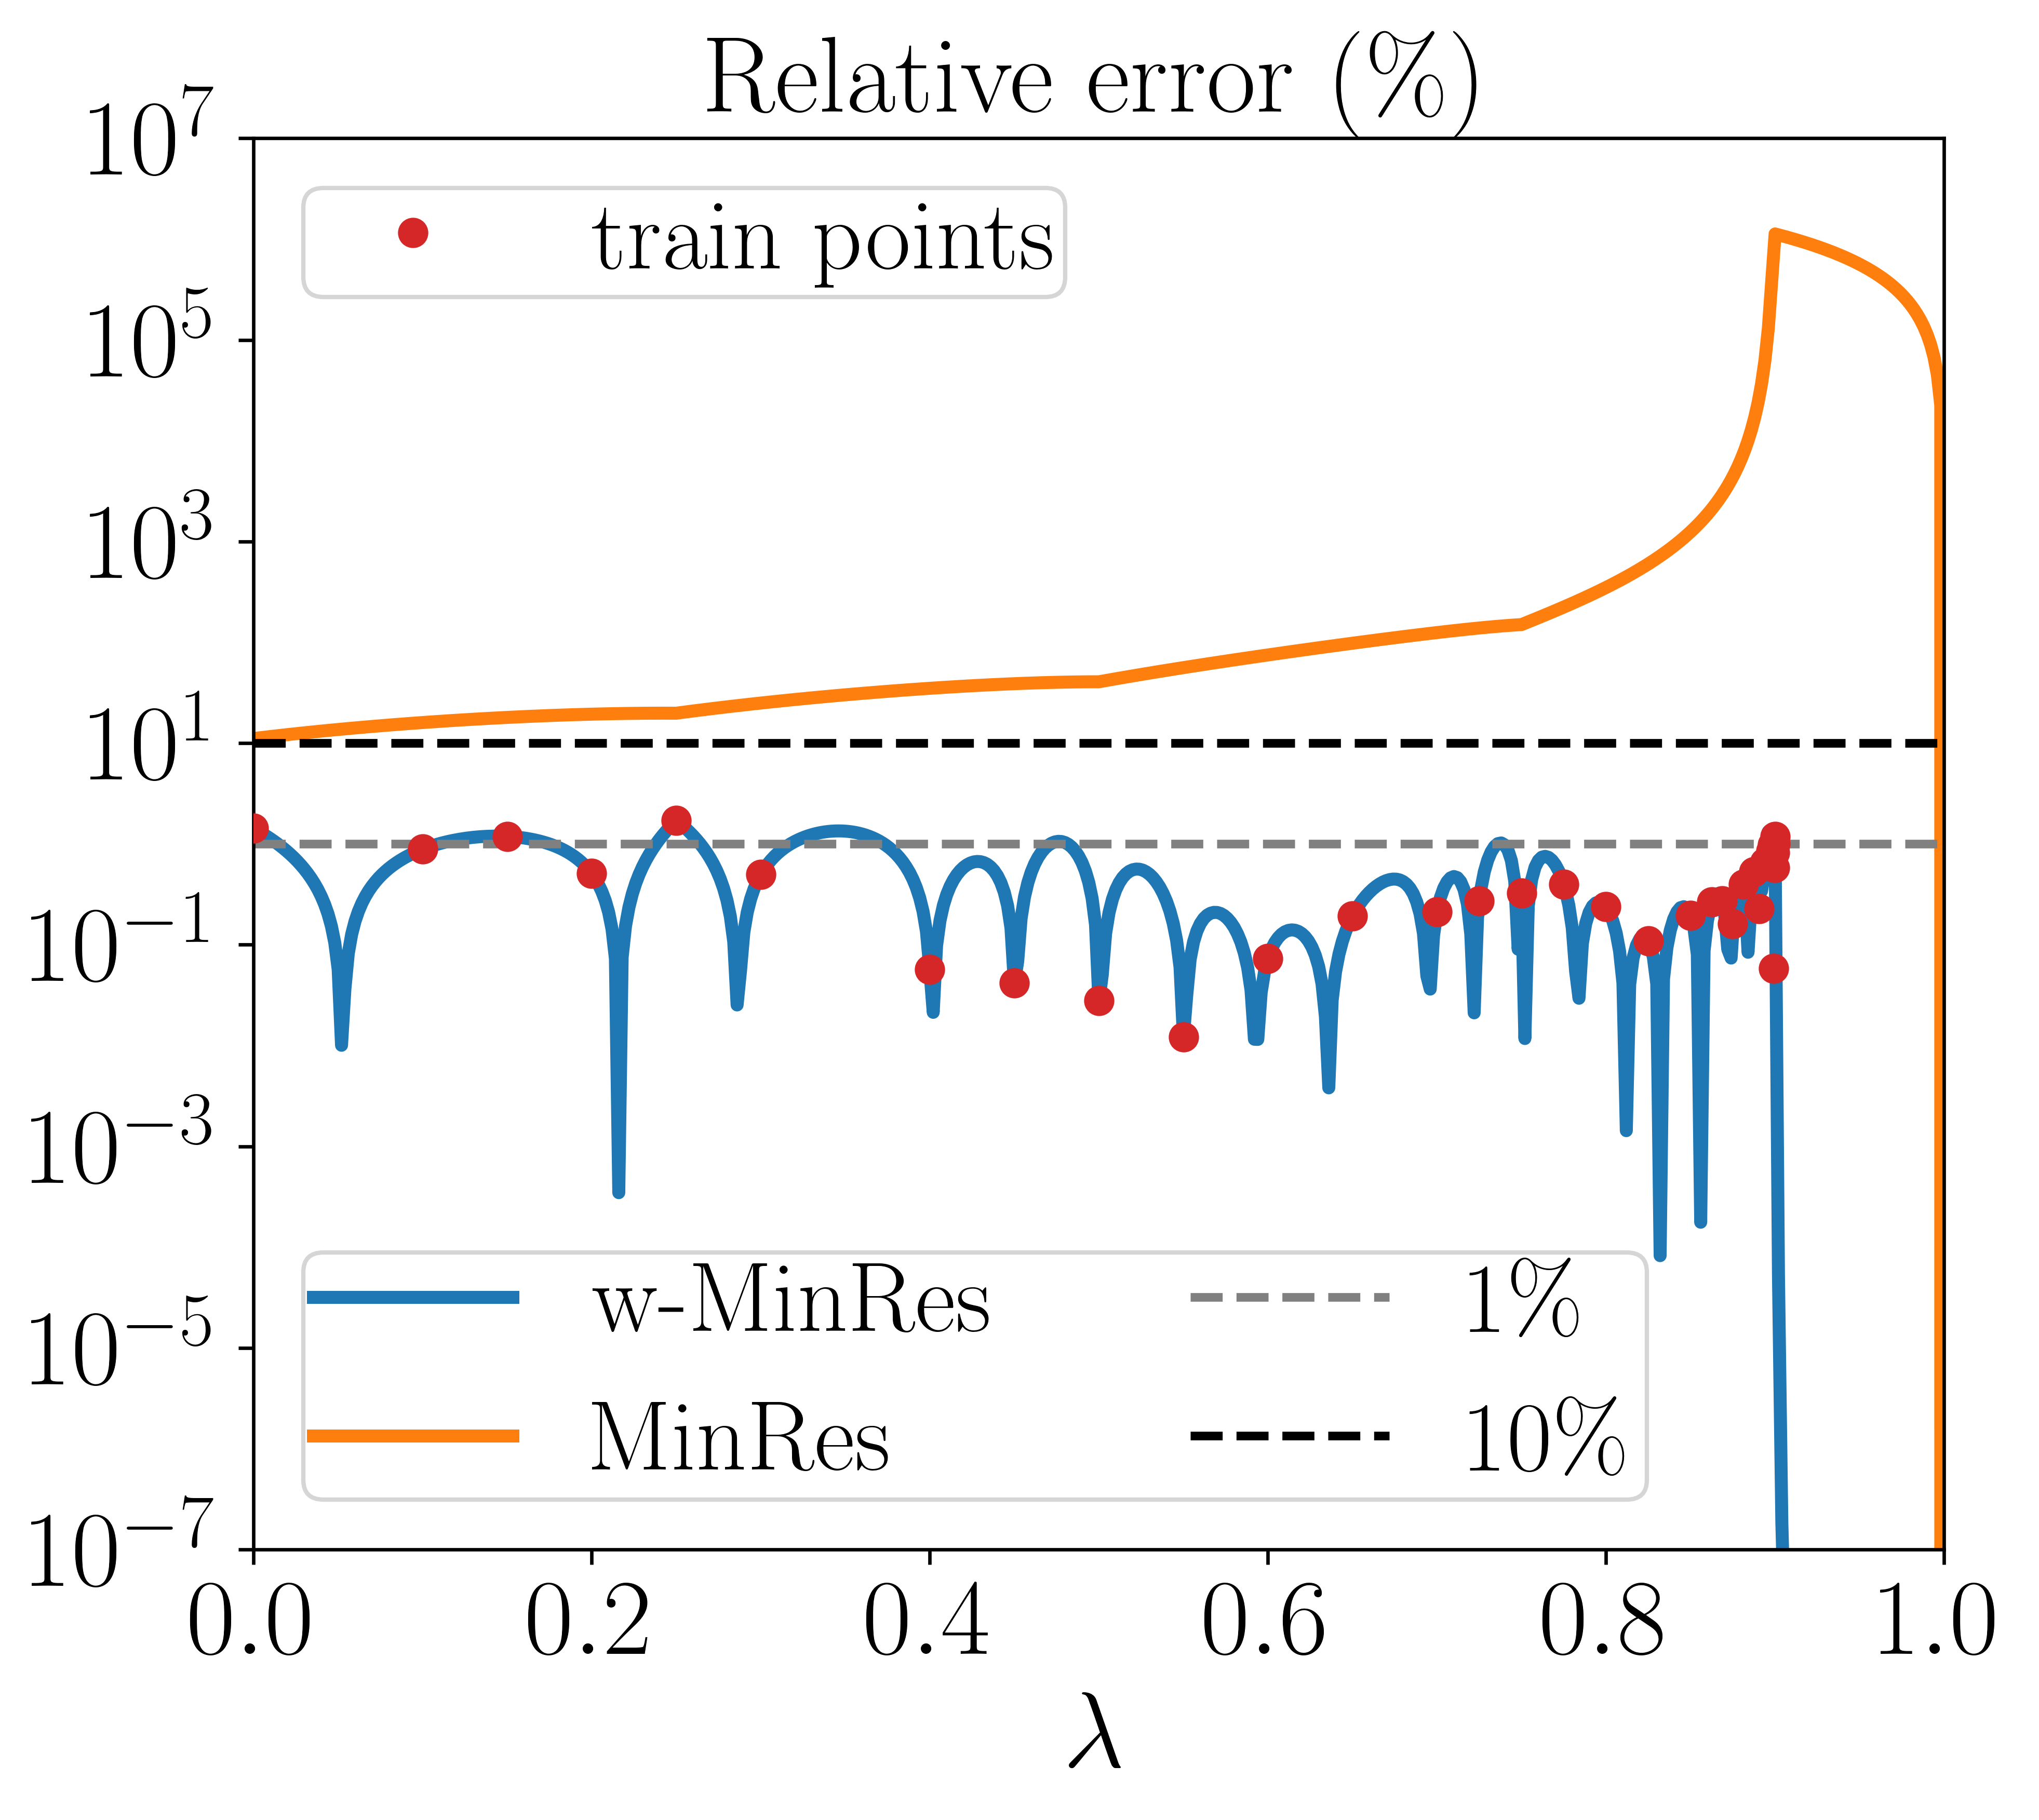
\includegraphics[scale=1.1]{Figures/ex2_rel_error_v2_latex_12_POSTER_v2.png}
}

%\block{Final $hp$-adapted meshes for Poisson example}{%
%\plothp{CrossGOA}
%}
%%%%%%%%%%%%%%%%%%%%%%%%%%%%%%%%%%%%%%%%%%%%%%%%%%%%%%%%%%%%%%%%%%%%%%%%%%
\block{References}{%
\begin{itemize}
\item[[$\,$1]] I. Brevis, I. Muga, and K.~G. van der Zee, \emph{A machine-learning minimal-residual (ML-MRes) framework for goal-oriented finite element discretizations}, Comput. Math. Appl., 95 (2021), pp. 186–199.
\item[[$\,$2]] I. Brevis, I. Muga, and K.~G. van der Zee, \emph{Neural control of discrete weak formulations: Galerkin, least-squares and minimal-residual methods with quasi-optimal weights}, Comput. Methods Appl. Mech. Engrg., 402 (2022), p. 115716.
\end{itemize}
}
\end{columns} 
% 

%\begin{columns}
%
%\column{0.25}
%\block{Formations}{
%\begin{itemize}
%\item Teaching (192h eq. TD in 2014-2015);
%\item Various formations on scientific computing (python, fortran, MPI);
%\item Languages certifications (DELE-C1 and CAE).
%\end{itemize}
%
%}
%\column{0.5}
%
%\block{Work in progress and future work}{
%\begin{itemize}
%\item Multi-D Goal-oriented Adaptivity;
%\item Theoretical proof of if there exists a $\hat{b}$ such that the alternative estimate is sharper than the classical one;
%\item Widen the study to other kind of problems (eg. diffusion-convection problems);
%\item Application to non-linear quantities of interest.
%\end{itemize}
%%
%}
%\column{0.25}
%
%
%\block{Mobility}{
%\begin{itemize}
%\item Bilbao (18 months);
%\item Pau (12 months);
%\item Valparaiso (6 months).
%\end{itemize}
%%
%}
%
%\end{columns} 

%\note[targetoffsetx=-3cm, targetoffsety=-2cm, angle=0, radius=0cm,width=7cm, rotate=10, connection, linewidth=.2cm,
%     roundedcorners=30, innersep=1cm]{\centering\vspace{1.5cm}\textbf{Published!}
%\scriptsize
%%Felipe V. Caro and Vincent Darrigrand and Julen Alvarez-Aramberri and Elisabete Alberdi and David Pardo.\\
%%A painless multi-level automatic goal-oriented $hp$-adaptive coarsening strategy for elliptic and non-elliptic problems.\\
%{\em Computer Methods in Applied Mechanics and Engineering}, 2022.
% }
\end{document}
